\section*{Question 3}
\begin{minipage}{0.5\textwidth}
A parallel‑plate capacitor with circular plates of radius $R$ and separation $d$ is being charged by a time‑varying conduction current
\[
I(t) = I_0 \sin(\omega t) \text{,}
\]
through connecting wires, where $I_0$ is a constant and $\omega \ll 1$ is the angular frequency of the current. The region between the plates is vacuum and $d \ll R$ so that the electric field between the plates is approximately uniform.
\end{minipage}
\begin{minipage}{0.5\textwidth}
    \centering
    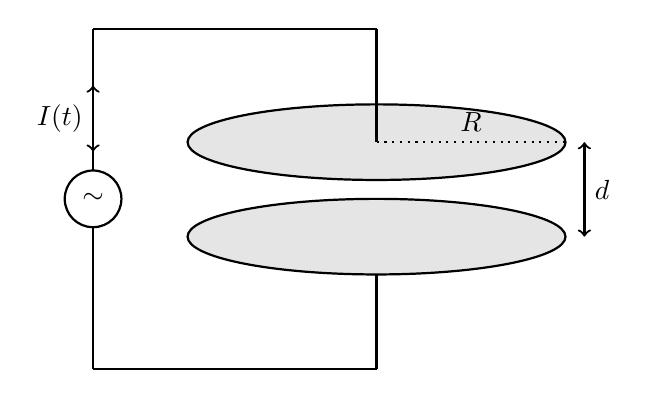
\begin{tikzpicture}[scale=1.2]
        % Plates
        \fill[gray!20] (-2,1) ellipse (2 and 0.4);
        \fill[gray!20] (-2,0) ellipse (2 and 0.4);
        \draw[thick] (-2,1) ellipse (2 and 0.4);
        \draw[thick] (-2,0) ellipse (2 and 0.4);

        % Wires
        \draw[thick] (-2,1.0) -- (-2,2.2);
        \draw[thick] (-2,-1.4) -- (-2,-0.4);
        \draw[thick] (-2,-1.4) -- (-5,-1.4);
        \draw[thick] (-2,2.2) -- (-5,2.2);
        \draw[thick] (-5,2.2) -- (-5,0.7);
        \draw[thick] (-5,0.1) -- (-5,-1.4);
        \draw[<->,thick] (-5,0.9) -- (-5,1.6) node[midway,left] {$I(t)$};

        \draw[<->, thick] (0.2,0) -- (0.2,1.0) node[midway,right] {$d$};

        % AC oscillator (circular)
        \draw[thick] (-5,0.4) circle (0.3) node {$\sim$};

        % Radius indicator
        \draw[dotted, thick] (-2,1.0) -- (0,1.0) node[midway,above] {$R$};
    \end{tikzpicture}
\end{minipage}
\begin{enumerate}
    \item[(a)] Write down the expression for the electric field $E(t)$ between the plates for as a function of instantaneous charge $Q(t)$ and $R$. --- \textit{0.2 pts}
    \item[(b)] Calculate the charge $Q(t)$ on the plates by using the integral $Q(t) = \int_0^t I(t') dt'$ and express $E(t)$ in terms of $I_0$, $R$ and $\omega$. --- \textit{0.3 pts} 
    \item[(c)] Using $\vec{J}_D=\epsilon_0 \frac{\partial \vec{E}}{\partial t}$, find the magnitude of the displacement current density $J_D(t)$ between the plates. What do you get if you consider the multiplication $J_D \pi R^2$? Would you expect it? Explain it briefly. --- \textit{0.2 pts}
    \item[(d)] Use the Ampère-Maxwell law $\oint \vec{B} \cdot d\vec{l} = \mu_0 \left( I_\text{enc} + \epsilon_0 \frac{d\Phi_E}{dt} \right)$ with a circular integration path of radius $r$ (centered on the axis, lying in a plane midway between the plates) to derive an expression for the magnetic field $B(r,t)$ for $r \leq R$. --- \textit{0.3 pts}
\end{enumerate}

\section*{Solution:}

\begin{solution}
(a) The electric field $E(t)$ between the plates of a parallel-plate capacitor is related to the charge $Q(t)$ on the plates by the formula:
\[
\boxed{
E(t) = \frac{\sigma}{\epsilon_0} = \frac{Q(t)}{\epsilon_0 A}= \frac{Q(t)}{\epsilon_0 \pi R^2}
}
\]
\noindent
(b) The instantaneous charge $Q(t)$ is given by the integral of the current $I(t)$ over time:
\[Q(t) = \int_0^t I(t') dt' = \int_0^t I_0 \sin(\omega t') dt' = \frac{I_0}{\omega} \left(1 - \cos\omega t\right)\]
Substituting this expression for $Q(t)$ into the formula for the electric field, we get:
\[
\boxed{
E(t) = \frac{I_0}{\epsilon_0 \pi R^2 \omega} \left[1 - \cos(\omega t)\right]
}
\]
\noindent
(c) The displacement current density $J_D(t)$ is related to the time derivative of the electric field by:
\[
\boxed{
J_D(t) = \epsilon_0 \frac{\partial E(t)}{\partial t}=\frac{I_0}{\pi R^2} \sin(\omega t)
}
\]
The multiplication $J_D \pi R^2$ gives:
\[J_D \pi R^2 = I_0 \sin(\omega t)\]
This represents the displacement current flowing through the area of the capacitor plates, which is equal to the conduction current $I(t)$ at any instant. It is expected because the displacement current density is defined such that it accounts for the changing electric field in the capacitor, which is necessary to maintain continuity of current in the circuit, especially when the conduction current is not present.

\noindent
(d) To find the magnetic field $B(r,t)$ for $r \leq R$, let us start with calculating the electric flux for Ampère-Maxwell law:
\[
\Phi_E = \int \vec{E} \cdot d\vec{A} = E(t) \cdot \pi r^2
\]
Thus, we have:
\[
\frac{d\Phi_E}{dt} = \frac{d}{dt} \left( E(t) \cdot \pi r^2 \right) = \pi r^2 \frac{dE(t)}{dt}
\]
Substituting this into the Ampère-Maxwell law, and considering the conduction current inside the capacitor is zero, we get:
\[
\oint \vec{B} \cdot d\vec{l} = \mu_0 \left( 0 + \epsilon_0 \pi r^2 \frac{dE(t)}{dt} \right) = \mu_0 \epsilon_0 \pi r^2 \left(\frac{dE(t)}{dt}\right)
\]
The left-hand side is $\oint \vec{B} \cdot d\vec{l} = B(r,t) \cdot 2\pi r$, the expression becomes:
\[B 2 \pi r = \mu_0 \epsilon_0 \pi r^2 \left( \frac{I_0}{\epsilon_0\pi R^2}\sin\omega t\right)\]
After simplifying, and rearranging the terms, we find:
\[\boxed{
B(r,t) = \frac{\mu_0 I_0}{2\pi R^2} r \sin(\omega t) \text{ for } r \leq R
}\]
\end{solution}
